This chapter first outlines the theoretical framework together with necessary data.
After that, the implementation is explained with references to methodological implications of the choices made.

\section{Requirements}
\label{sec:requirements}
A series of tools will help to achieve lexicalized tokenization.
They will be explained in this section along with their methodological edge.

\subsection{Pipeline Structure \& Transformers Library}
\label{subsec:architecture}

\ac{bert} is a language learning transformer model designed for \ac{nlp} tasks (\cite{ATTENTION}).
Upon release it achieved higher performance scores compared to previously used \ac{lstm} models (\cite{BERTHIGH1}).
Two main model characteristics can be observed for \ac{bert}.
Firstly, it is the first \ac{lm} to implement simultaneous attention heads, allowing for bidirectional reading.
The methodological implication of reading to the left and right of a token is to include more information about the language in single embeddings.
Secondly, \ac{bert} introduced the (at the time novel) \ac{mlm} method for training.
The method involves masking a specified amount (default 15\%) of random tokens in the input sequence.
Masked tokens are guessed by the model which can then update its weights according to success or failure.

The \ac{nlp} community has since developed \ac{bert} and adapted it to the needs of contemporary \ac{nlp} problems (e.g. \ roberta, germanbert, mbert).
Its wide support, comparability and versatility make \ac{bert} the model of choice for this thesis.
Another notable feature in \uppercase{bert} is the implementation of the WordPiece tokenizer module\footnote{The source code was not published but is inferred on \href{https://huggingface.co/course/chapter6/6?fw=pt}{huggingface}}.
Default BERT WordPiece tokenization is predominantly heuristic by combining strings based on a precalculated score.
A variety of pre-trained tokenizers are available, although they come with a caveat.
Once a tokenizer is trained on a dataset it is specific to that dataset.
This means the application of a tokenizer on another dataset may result in out-of-vocabulary issues and different token/subtoken distributions.

Particularly relevant to this thesis is the option to train an own tokenizer from the base module.
Usually, WordPiece generates its own set of subtokens called \textit{vocabulary}, which is used by the standard tokenizer to generate unique numerical input IDs.
These identifiers correspond to tokens or parts of tokens found in the original dataset that the model was trained on.
Wordmap partly takes over the tokenization depending on the the type of input it receives, the exact process is given in \autoref{subsec:tokenizer}.
Once a string is tokenized it gets passed on to the transformer model for contextualized embedding.
\autoref{fig:pipeline} shows the processing of data up until token encoding.

\begin{figure}
    \centering

    \tikzset{every picture/.style={line width=0.75pt}} %set default line width to 0.75pt

    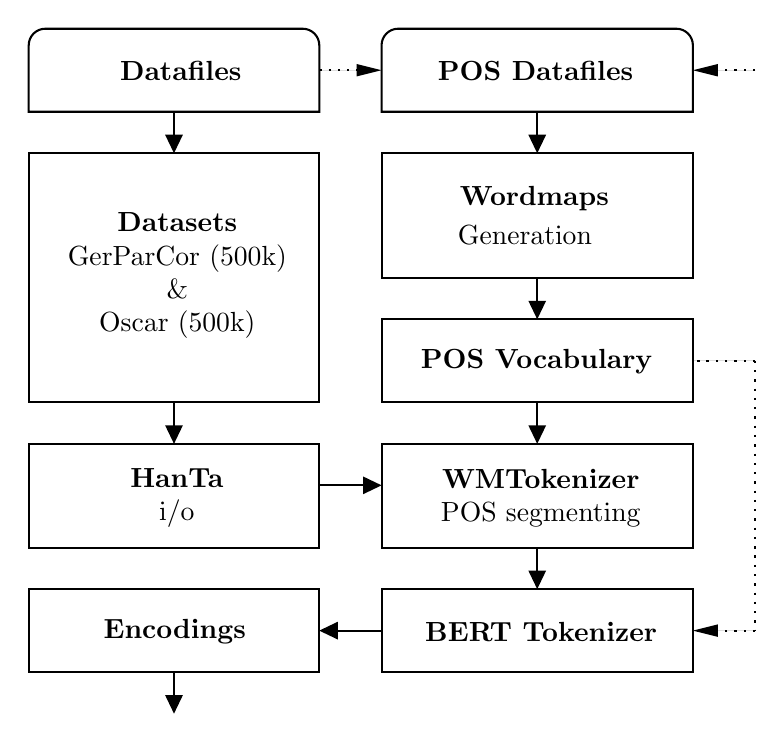
\begin{tikzpicture}[x=0.75pt,y=0.75pt,yscale=-1,xscale=1]
        \draw   (40,98) .. controls (40,93.58) and (43.58,90) .. (48,90) -- (172,90) .. controls (176.42,90) and (180,93.58) .. (180,98) -- (180,130) .. controls (180,130) and (180,130) .. (180,130) -- (40,130) .. controls (40,130) and (40,130) .. (40,130) -- cycle ;
        \draw   (210,98) .. controls (210,93.58) and (213.58,90) .. (218,90) -- (352,90) .. controls (356.42,90) and (360,93.58) .. (360,98) -- (360,130) .. controls (360,130) and (360,130) .. (360,130) -- (210,130) .. controls (210,130) and (210,130) .. (210,130) -- cycle ;
        \draw   (210,150) -- (360,150) -- (360,210) -- (210,210) -- cycle ;
        \draw   (210,230) -- (360,230) -- (360,270) -- (210,270) -- cycle ;
        \draw   (40,150) -- (180,150) -- (180,270) -- (40,270) -- cycle ;
        \draw   (40,290) -- (180,290) -- (180,340) -- (40,340) -- cycle ;
        \draw   (210,290) -- (360,290) -- (360,340) -- (210,340) -- cycle ;
        \draw   (210,360) -- (360,360) -- (360,400) -- (210,400) -- cycle ;
        \draw [fill={rgb, 255:red, 0; green, 0; blue, 0 }  ,fill opacity=1 ] [dash pattern={on 0.84pt off 2.51pt}]  (390,110) -- (362,110) ;
        \draw [shift={(360,110)}, rotate = 360] [fill={rgb, 255:red, 0; green, 0; blue, 0 }  ][line width=0.08]  [draw opacity=0] (12,-3) -- (0,0) -- (12,3) -- cycle    ;
        \draw    (285,130) -- (285,147) ;
        \draw [shift={(285,150)}, rotate = 270] [fill={rgb, 255:red, 0; green, 0; blue, 0 }  ][line width=0.08]  [draw opacity=0] (8.93,-4.29) -- (0,0) -- (8.93,4.29) -- cycle    ;
        \draw    (110,130) -- (110,147) ;
        \draw [shift={(110,150)}, rotate = 270] [fill={rgb, 255:red, 0; green, 0; blue, 0 }  ][line width=0.08]  [draw opacity=0] (8.93,-4.29) -- (0,0) -- (8.93,4.29) -- cycle    ;
        \draw    (110,270) -- (110,287) ;
        \draw [shift={(110,290)}, rotate = 270] [fill={rgb, 255:red, 0; green, 0; blue, 0 }  ][line width=0.08]  [draw opacity=0] (8.93,-4.29) -- (0,0) -- (8.93,4.29) -- cycle    ;
        \draw    (285,210) -- (285,227) ;
        \draw [shift={(285,230)}, rotate = 270] [fill={rgb, 255:red, 0; green, 0; blue, 0 }  ][line width=0.08]  [draw opacity=0] (8.93,-4.29) -- (0,0) -- (8.93,4.29) -- cycle    ;
        \draw    (285,270) -- (285,287) ;
        \draw [shift={(285,290)}, rotate = 270] [fill={rgb, 255:red, 0; green, 0; blue, 0 }  ][line width=0.08]  [draw opacity=0] (8.93,-4.29) -- (0,0) -- (8.93,4.29) -- cycle    ;
        \draw    (285,340) -- (285,357) ;
        \draw [shift={(285,360)}, rotate = 270] [fill={rgb, 255:red, 0; green, 0; blue, 0 }  ][line width=0.08]  [draw opacity=0] (8.93,-4.29) -- (0,0) -- (8.93,4.29) -- cycle    ;
        \draw    (180,310) -- (207,310) ;
        \draw [shift={(210,310)}, rotate = 180] [fill={rgb, 255:red, 0; green, 0; blue, 0 }  ][line width=0.08]  [draw opacity=0] (8.93,-4.29) -- (0,0) -- (8.93,4.29) -- cycle    ;
        \draw [fill={rgb, 255:red, 0; green, 0; blue, 0 }  ,fill opacity=1 ] [dash pattern={on 0.84pt off 2.51pt}]  (180,110) -- (208,110) ;
        \draw [shift={(210,110)}, rotate = 180] [fill={rgb, 255:red, 0; green, 0; blue, 0 }  ][line width=0.08]  [draw opacity=0] (12,-3) -- (0,0) -- (12,3) -- cycle    ;
        \draw   (40,360) -- (180,360) -- (180,400) -- (40,400) -- cycle ;
        \draw    (210,380) -- (183,380) ;
        \draw [shift={(180,380)}, rotate = 360] [fill={rgb, 255:red, 0; green, 0; blue, 0 }  ][line width=0.08]  [draw opacity=0] (8.93,-4.29) -- (0,0) -- (8.93,4.29) -- cycle    ;
        \draw [fill={rgb, 255:red, 65; green, 183; blue, 159 }  ,fill opacity=0.79 ]   (110,400) -- (110,417) ;
        \draw [shift={(110,420)}, rotate = 270] [fill={rgb, 255:red, 0; green, 0; blue, 0 }  ][line width=0.08]  [draw opacity=0] (8.93,-4.29) -- (0,0) -- (8.93,4.29) -- cycle    ;
        \draw  [dash pattern={on 0.84pt off 2.51pt}]  (390,250) -- (390,380) ;
        \draw [fill={rgb, 255:red, 0; green, 0; blue, 0 }  ,fill opacity=1 ] [dash pattern={on 0.84pt off 2.51pt}]  (390,380) -- (362,380) ;
        \draw [shift={(360,380)}, rotate = 360] [fill={rgb, 255:red, 0; green, 0; blue, 0 }  ][line width=0.08]  [draw opacity=0] (12,-3) -- (0,0) -- (12,3) -- cycle    ;
        \draw [fill={rgb, 255:red, 0; green, 0; blue, 0 }  ,fill opacity=1 ] [dash pattern={on 0.84pt off 2.51pt}]  (390,250) -- (360,250) ;
        \draw (111.6,209) node   [align=left] {\begin{minipage}[lt]{83.78pt}\setlength\topsep{0pt}
        \begin{center}
            \textbf{Datasets}\\GerParCor (500k)\\\&\\Oscar (500k)
        \end{center}
        \end{minipage}};
        \draw (113.27,110.5) node   [align=left] {\textbf{Datafiles}};
        \draw (284.19,110.5) node   [align=left] {\textbf{POS Datafiles}};
        \draw (283.62,180) node   [align=left] {\begin{minipage}[lt]{55.24pt}\setlength\topsep{0pt}
        \begin{center}
            \textbf{Wordmaps}
        \end{center}
        Generation
        \end{minipage}};
        \draw (284.8,250.5) node   [align=left] {\textbf{POS Vocabulary}};
        \draw (286.7,316) node   [align=left] {\begin{minipage}[lt]{88.34pt}\setlength\topsep{0pt}
        \begin{center}
            \textbf{WMTokenizer}\\POS segmenting
        \end{center}
        \end{minipage}};
        \draw (286.87,380.5) node   [align=left] {\textbf{BERT Tokenizer}};
        \draw (111.37,316) node   [align=left] {\begin{minipage}[lt]{56.94pt}\setlength\topsep{0pt}
        \begin{center}
            \textbf{HanTa}\\ i/o
        \end{center}
        \end{minipage}};
        \draw (110.34,380.5) node   [align=left] {\textbf{Encodings}};

    \end{tikzpicture}
    \caption[Schematic integration of Wordmap segmentation into the BERT architecture.]{Schematic integration of Wordmap segmentation into the BERT architecture. Continuous lines show non-selective channels, while dotted lines only pass data selectively}
    \label{fig:pipeline}
\end{figure}

In \autoref{fig:pipeline}, Datafiles contains the raw unprocessed data coming from corpora.
The input is provided in txt-files holding sentences line by line.
Two datasets are generated from this input, each amounting to 500000 sentences per corpus for fine-tuning.
POS Datafiles ideally contains only words that are identified as the same \ac{pos} category.
To increase the resulting POS vocabulary, POS Datafiles can be augmented by two channels: input can come from the corpus itself, but would need to be tagged first.
Otherwise a predefined list of words can be used as an external and generic source for Wordmap generation.
In POS Vocabulary, adjustments like removing outliers and interferences are performed on the set of subwords yielded by Wordmap generation.
It is important to note that the POS vocabulary is separate from the the tokenizer vocabulary.
This serves the specific purpose of keeping the vocabulary on which the model is trained clean from unwanted or unused subwords.
Machine learning practice generally points to the trade-off between vocabulary size and model performance, hence the addition of POS Vocabulary to the BERT Tokenizer vocabulary is used only when necessary.
Datasets are then passed through \ac{hanta} to provide WMTokenizer with flagged data to tokenize only selected tokens.
Lastly BERT Tokenizer returns the current standard encodings used in \ac{bert} language modeling.

\subsection{Data}
\label{subsec:data}
Two corpora where selected for fine-tuning: \ac{gerparcor} and oscar (\cite{oscar}).
FLOTA was trained on 12000 samples per  category ~\cite{FLOTA}, which is why for this fine-tuning a sample size of 500000 seems sufficient.
GerParCor is a \enquote{GerParCor genre-specific corpus of (predominantly historical) German-language parliamentary protocols from three centuries and four countries, including state and federal level data.} (\cite[1]{GERPARCOR}).
Of all subcorpora included in \ac{gerparcor}, one specifically texts and transcripts of the german parliament.
All 500k samples in the \ac{gerparcor} dataset used for this thesis are found in the \texttt{Bundestag} subcorpus of \ac{gerparcor}.
Oscar offers other subcorpora partly hosted on huggingface.
In this case, a web-crawled german corpus called \texttt{unshuffled\_deduplicated\_de} was chosen, as introduced by its curators (\textcite{oscarsub2}; (\textcite{oscarsub1}).

The POS vocabulary put throuh the Wordmapping pipelines comes from ~\textcite{wiktionary} and \ac{hanta}-crawled verbs of gerparcor ~\cite{hanta}


\section{Implementation}
\label{sec:implementation}

The implementation of aforementioned methodology is presented in this section.
The core part is the conceptualization and implementation of the tokenizer, which is explained in three steps:
the wordmap algorithm generating a vocabulary, the segmentation algorithm for token segmentation and maximization, and the integration into \ac{bert}.
After that a short description of model hyperparameterization and training is given.
The same is done for the model evaluation task in the last subsection of this chapter.

\subsection{Tokenizer}
\label{subsec:tokenizer}
The methods of tokenization are explained in the following subsection.
This is also the main part of the thesis, containing two algorithms - one for vocabulary generation and one for token segmentation.
Throughout this section, the words $target$ and $token$ are used to describe a word that is analyzed.
One denotes the argument of the wordmapping and segmenter function ($target$), the other describes a word occurring in the corpus ($token$).

\subsubsection{Generating a custom pre-training vocabulary}
\label{subsubsec:generating-a-custom-pre-training-vocabulary}

Embedding those subwords which take part in inflectional processes essentially means deriving sensible subwords to represent actual morphemes.
The vocabulary generated for this chapter is a list of inflected and non-inflected verbs (as to state the example) provided by two sources: (1) the german verb wiktionary and (2) a crawl of the GerParCor corpus with the HanTa tagger \cite{hanta}.
Initial experiments where done only with the wiktionary verb list since it provided sanitized input for the algorithm in development.
As soon as the verbs where extracted from \ac{gerparcor} via \ac{hanta} they where added to increase the sample size at the cost of adding noise.
A naive regular expression detecting syllable nuclei was used to sort the verbs into their respective syllable count.
It provides an overview over the POS dataset and can potentially decrease iterations.
The whole POS dataset was iterated over nevertheless, words with syllable count 2 or less are only analyzed to the right to prevent the algorithm from analyzing words that are likely to not have a prefix.
Through the positional distribution and morphological variety mentioned in \autoref{sec:target-languages} this did not pose a problem.

The Wordmap algorithm as shown in \autoref{alg:wordmap} is the first step to extracting morphemes from a token.
Its purpose is to compare two strings and store their intersections in a map of boolean values.

\algrenewcommand\algorithmicrequire{\textbf{Input:}}
\algrenewcommand\algorithmicensure{\textbf{Output:}}
\begin{algorithm}
    \caption{Wordmap generation}\label{alg:wordmap}
    \begin{algorithmic}[1]
        \Require $verbs = \{v : \uppercase{POS}\}, target$ \Comment{\textit{verbs}: set of single-\uppercase{POS} lexemic tokens}
        \Ensure $maps = (map_{1}, \ldots, map_{|verbs|})$
        \Function{wordmap}{w1, w2, \*d=0}
            \State $f_{1}: c1, c2 \mapsto c1 == c2$
            \State $f_{2}: \left(\sum_{i=0+d}^{\mid w1 \mid} w1[i], w2[i] \mapsto f_{1}(w1[i], w2[i])\right)$
            \State \textbf{return} $f_{2}$
        \EndFunction
        \\

        \For{$v \in verbs$}
        \State $pair = (target, v)$
        \State $s = \textsc{shorter}(pair)$
        \State $l = \textsc{longer}(pair)$
        \State $case = \textsc{match\_ends}(pair)$ \Comment{Returns if strings match in the last or first position}
        \State $len = \textsc{len}(l)$
        \State $\delta = \Delta(len, \textsc{len}(s))$
        \\

        \If{$\textit{case: any match}$}
            \If{$\delta$}
                \If{$\textit{case: left match}$}
                        \State $\textsc{wordmap}(l, s)$
                    \State Pad map from right side with 0s to match $len$
                \EndIf
                \If{$\textit{case: right match}$}
                        \State $\textsc{wordmap}(l, s, \delta)$
                    \State Pad map from left side with 0s to match $len$
                \EndIf
            \Else
                \State $\textsc{wordmap}(l, s)$
            \EndIf
        \EndIf
        \EndFor

    \end{algorithmic}
\end{algorithm}

% DESCRIPTION OF ALGORITHM 1

Wordmap requires two \textbf{inputs} $verbs$ and $target$.
The resulting wordmap will be generated for $target$, while $verbs$ serves as comparison.
Any map generated from this also has the same length as $target$.
$verbs$ is a set of tokens pertaining to the same \ac{pos} category.
Note that $verbs$ should only contain those POS-tagged tokens that are expected to carry lexical information (e.g.\ verbs, adjectives, etc.).
The set is previously extracted from the corpus by \ac{pos}\hyphen tagging.
Optionally, the set can be augmented by manually adding \ac{pos} matching tokens from external sources.
The 2-tuple $pair$ are the strings to be compared.
It is passed on to (1) \textsc{shorter}, a function returning the shorter of both strings (2) \textsc{longer}, expectedly returning the longer of both strings (3) \textsc{match\_case}, a function to determine the behavior of the algorithm later on.
As two strings are compared \textsc{match\_case} captures three cases: $pair$ matches in the first, last or both positions.
Finally $len$ denotes the length of the longest string and $\delta$ difference in length between $s$ and $l$.
$\delta$ functions as an offset for index-based comparisons \textsc{wordmap}, the mapping function generating the Wordmaps.

Once every $v$ has been compared to $target$, $maps$ stores boolean counts of characters occurring in their respective positions in $target$.
Every map is cleaned with a regular expression to reduce noise caused by natural character occurrence (some characters like \textless n\textgreater, \textless s\textgreater ~will be more frequent than others).
Omitting this step will result cause a ceiling effect rendering the maps useless.
Continuous concatenations of leading or trailing matches stay, while every match enclosed by $0$ will be replaced the $0$.
As an example, $wordmap = 11101100101$ contains three matches on the inside which will result in $11100000001$ as final output.
In the penultimate stage of mapping $target$, all maps are summed up to receive the number of absolute positional occurrences of every character in $target$.
This positional mapping allows for detecting relevant segments in a token based on a threshold.
Characters in range of the predefined threshold are selected for the mapping of a target token.
Functional morphemes (morphemes that are carriers of grammatical features) are typically much more frequent than their lexical counterparts.
Consequently, lexical morphemes in the family of inflectional languages are - by definition - modified by functional morphemes, they occur much less frequently.
In this case, the activation function for a concatenation of same boolean values to be selected as segment is the normalizing z-score function defined as: $z_{i} = \frac{x_{i} - \overline{x}}{S}$,
where $z$ is the z-score, $\overline{x}$ and $S$ are the sample mean and the sample standard deviation.
Any segment below a z-score of zero is detected.
For every verb that is mapped, the detected affixes are added to a vocabulary of functional morphemes.
The rest of the string is saved into the vocabulary of lexemic segments, assuming that it still contains the lexical information in the verb.

\begin{table}[H]
    \centering
    \caption{Example Wordmaps for $target = \texttt{verstehen}$}
    \label{tab:wordmaps}
    \begin{tabular}{llll}
        \toprule
        \textbf{String} & \textbf{Wordmap} & \textbf{Case} & \textbf{Padding} \\
        \midrule
        \texttt{verarbeiten} & 111000000 & left match & Yes \\
        & 001000011 & right match & Yes \\
        \texttt{variiert} & 101001000 & left match & Yes \\
        \texttt{vormachen} & 101000111 & left match & No \\
        & 101000111 & right match & No \\
        \texttt{anstrebtest} &  & no match &   \\
        (...) &  &  &  \\
        \bottomrule
    \end{tabular}
\end{table}

Both vocabularies are then cleared of outliers in different ways.
The functional vocabulary drops every string longer than 2.5 times the standard deviation of its own population.
Since more variance in length is expected in the lexemic vocabulary, the outlier function is limited to drop everything above the length  of 2 times the mean absolute deviation as a staple method for more volatile datasets.
The upper segment of n-length strings in the lexemic vocabulary has thus been covered, but the low segment (short strings) remains untouched.
To solve this problem, probably one of the more reaching but important measures is taken: removing any string of the lexemic vocabulary that is smaller than the mean length of strings in the functional vocabulary.
Removing this interference in vocabularies is subject to the notion that functional morphemes will be shorter than lexemic morphemes.
After minimizing outliers and interference, both vocabularies are joined again to form the segmenters vocabulary.

\subsubsection{BERT Tokenizer Modification}
\label{subsubsec:tokenizer-modification}
The BERT tokenizer module tokenizes using subwords form its own vocabulary during pre-training.
By loading the \ac{bbgc} pre-trained tokenizer with and an instance of \ac{hanta} as taggint overhead a sample from the dataset batching function can be fully encoded for training.
While iterating over the sample \ac{hanta} passes on detected verbs to \autoref{alg:segmenter}.
All tokenized subsentences are then joined and added to the encoded batch.

\begin{algorithm}
    \caption{Target Segmentation}\label{alg:segmenter}
    \begin{algorithmic}[1]
        \Require $target,pos\_vocab$ \Comment{Vocabulary consisting of verbs only}
        \Ensure $\{(tuples\:of\:subwords)\} \approx \{ t \in \mathcal{P} (s \in pos\_vocab : s \in target) : t \equiv target\}$
        \\
        \State $segmentations = ()$
        \\

        \Function{segmenter}{token, stop, start=0, segments}
        \If{$start = stop$}
            \State Add $segments$ to $segmentations$
        \Else
            \State $morphemes = (m \in pos\_vocab : target. \textsc{startswith}(m) \wedge |m|>1)$
            \For{$m \in morphemes$}
                \State $start \mathrel{+}= \textsc{len}(m)$
                \State Add $m$ to $segments$
                \State $rest = target[\textsc{len}(m):]$
                \If{$\textsc{len}(rest)==1$}
                    \State $start = stop$
                    \State Add $rest$ to $segments$
                    \State Add $segments$ to $segmentations$
                    \State Decrement $start$, crop $segments$
                \Else
                    \State $\textsc{segmenter}(target=rest, stop, start=start, segments)$
                    \State Decrement $start$, crop $segments$
                \EndIf
            \EndFor
        \EndIf
        \EndFunction
        \State $\textsc{maximize\_segments}(segmentations)$
    \end{algorithmic}
\end{algorithm}

\autoref{alg:segmenter} recursively computes every possible segmentation for a string $target$ from a given vocabulary $pos\_vocab$ from left to right.
The vocabulary contains all the segments that were identified in the previous step by \autoref{alg:wordmap}.
Every segmentation has to be complete so that its segments corresponds to non overlapping substrings of $target$.
For every $target$ a subvocabulary $morpheme$ is defined, containing all strings that are in the vocabulary of \ac{POS} \- members.
This task is a weighted coverage problem in the \uppercase{NP}-hard domain.
Unary morphemes to the left are excluded from the pre-selected subvocabulary to drastically reduce the number of possible permutations , as they can be embedded in n-ary tokens as well.
The recursion can be seen as n-ary a trees containing every permutation of the set $morphemes$ where the sum of branches all satisfy $target$.

\begin{figure}
\centering
\begin{forest}
    for tree={
        grow=south,
        minimum size=2ex, inner sep=1pt,
        s sep=7mm
    }
    [Call: & \textsc{segmenter}(\texttt{"verstehen"})\\\hline
    Subvocab: & \{\texttt{versteh\, vers\, ver\, ve\, en\, teh\, \, steh\, ste\, st\, rsteh\, rst\, rste\, ehe\, he\, n\}}\\
    ,align=11,draw
    [{\texttt{verstehen}}
    [\texttt{versteh}
    [\texttt{en}]
    ]
    [\texttt{vers}
    [\texttt{teh}
    [\texttt{en}]]
    [\texttt{te}
        [\texttt{he}
        [\texttt{n}]]]]

    [\texttt{ver}, draw, dotted
    [\texttt{steh}, draw, dotted
    [\texttt{en}, draw, dotted
    ]
    ]
    [\texttt{ste}
    [\texttt{he} [\texttt{n}]]]
    [\texttt{st}
    [\texttt{ehe} [\texttt{n}]]
    [\texttt{eh} [\texttt{en}]]]
    ]
    [\texttt{ve}
    [\texttt{rsteh} [\texttt{en}]]
    [\texttt{rst}
    [\texttt{eh} [\texttt{en}]]
    [\texttt{ehe} [\texttt{n}]]
    ]
    [ \texttt{rste} [\texttt{he} [\texttt{n}]]]
    ]
    ]
    ]


\end{forest}
\caption[Segmenter output for \texttt{verstehen}]{Permutations \textsc{segmenter} generates from target i.e. \texttt{verstehen}. Dotted segments mark the segmentation chosen later by the maximization function during tokenization.}
\label{fig:segmentationtree}
\end{figure}

As shown in \autoref{fig:segmentationtree}, all morphemes that $target$ starts with are stored to form the first nodes of the permutation tree.
Each time a morpheme is selected the index $start$ is incremented by the length of the morpheme to indicate when the string has been completely segmented.
The new recursion is called with the updated index $start$ and $target$ sliced by the length of the morpheme contained in the parent node.
Incomplete segmentations that miss exactly one character to the right are accepted with the added missing string.
If the vocabulary cannot satisfy a segmentation because it is missing the necessary strings, segmentation is omitted and the original input token is returned as such.

Then, of all $segmentations$ a single segmentation is selected by a maximization function \textsc{maximize\_segments} calculating weights for every segment.
The maximization function for one segment is the defined as:

\begin{equation}\label{eq:maximization}
    \underset{s \in S}{\arg\max} f(s) \coloneqq  \Bigl\{ s \in S : \sum_{i=1}^{|s|} \sqrt[s_{i}]{\frac{s_{i}}{t} \div |s|}\Bigr\}
\end{equation}

Where $S$ is a set of segmentation tuples $s$, $|s|$ is the length of the tuple (read: number of segments) and $s_{i}$ indicates the length of the segment at position $i$ in tuple $s$.
For every segment (vertex) in a segmentation tuple (branch)  the segment's length is divided by the token length $t$ to get the coverage the morpheme provides towards the target string.
The number of segments $|s|$ is a divisor meant to cap the number of segments in a segmentation.
It prevents choosing a segmentation overflowing with too many short segments.
Short segments are convenient for completing a segmentation, but will increase the chance of slicing a token where it linguistically lacks sense to do so.
Lastly the $s_{i}$^{\text{th}} root implements a bias against segments that are too long.
While the accuracy decreases for longer words, this method of maximization performs reasonably well in the range of 1--4 syllable tokens, which make up around 87\% of the verb vocabulary.


Ultimately, segmentation is a matter of interpretation.
If there are several possible interpretations by wich to segment a word this tokenization method relies on the assumption that the comparison with \ac{pos}- members displays the probable shape of segmentation for a token.
As mentioned in~\ref{subsec:masked-language-model}, the default WordPiece Tokenizer lacks
A linguistically informed



The field of NLP  (\cite{METZLER2016}) has been expanded ever since the emergence of the language models.
Natural language processing is understood as the



\subsection{Model Training}
\label{subsec:masked-language-model}
All fine-tuned models use the \ac{bbgc} baseline by \textcite{bertbasegermancased}.
For reference and readability they are given shortened IDs as follows:\\

\begin{table}[h]
    \centering
    \caption{ID references assigned to full model names}
    \label{tab:modelids}
    \begin{tabular}{ll}
        \toprule
        \textbf{ID} & \textbf{Full name} \\
        \midrule
        mwg5 & mlm\_wmt\_gpc500k \\
        mwo5 & mlm\_wmt\_oscar500k \\
        msg5 & mlm\_std\_gpc500k \\
        mso5 & mlm\_std\_oscar500k \\
        bbgc & bert-base-german-cased \\
        \bottomrule
    \end{tabular}
\end{table}

The full model names in \autoref{tab:modelids} captures broad characteristics of the model.
For example, \fbox{mwo5} is the \fbox{m}asked language model using \fbox{W}ordmap tokenization fine-tuned on the \fbox{O}scar dataset of \fbox{5}00k samples, while msg5 is the the masked language model using standard BERT wordpiece tokenization fine-tuned on the GerParCor dataset of 500k samples.
All models except for bbgc are trained on the same parameters as seen in table \autoref{tab:modelshyper}.\\

\begin{table}[h]
    \centering
    \caption[List of all used models]{List of all used models and their hyperparameters. LR = learning rate, WU = warmup steps.}
    \label{tab:modelshyper}
    \begin{tabular}{lllrrrrl}
        \toprule
        \textbf{ID} & \textbf{Corpus} & \textbf{Tokenization} & \textbf{LR} & \textbf{Steps} & \textbf{Batchsize} & \textbf{WU} & \textbf{Base} \\
        \midrule
        mwg5 & GerParCor & BWP + WM & 0.0003 & 31250 & 16 & 500 & bbgc \\
        mwo5 & Oscar & BWP + WM & 0.0003 & 31250 & 16 & 500 &  bbgc \\
        msg5 & Gerparcor & BWP & 0.0003 & 31250 & 16 & 500 &  bbgc \\
        mso5 & Oscar & BWP & 0.0003 & 31250 & 16 & 500 &  bbgc \\
        bbgc & Mixed & BWP & 0.0001 & 810k/30k & 1024 & 10000 & - \\
        \bottomrule
    \end{tabular}
\end{table}

The first four models use bbgc as baseline, meaning that they inherit its structural properties.
DeepsetAI released bbgc training it in two phases (see column Steps in \autoref{tab:modelshyper}) with differing sequence lengths 128/512 respectively.
The maximum sequence length for each model is 512, the base vocabulary size is 30k.
Models mwg5, mwo5, msg5, and mso5 where trained with less steps and thus higher learning rate to converge quicker with the given datasets.
The models where implemented in PyTorch (\textcite{pytorch}) and trained on the GPUs Quadro RTX 8000 (48Gb) and NVIDIA GeForce GTX 1080 Ti (11Gb) provided at \ac{ttl}.

\subsection{Benchmark}
\label{subsec:benchmark-implementation}
The original draft for this thesis featured a benchmark with a translated multiple choice question answering task from the oLMpics benchmark (\cite{olmpics}).
Due to incompatible versioning dependencies this was not feasible and a substitute had to be found.
To test the performance of trained models a one-shot sequence classification task is set up instead.
The task consists of \textasciitilde11k samples containing a sentence and a single label.
Each sentence is the title of a news article found on the german Wikinews site, belonging to one of the categories listed on their topic section\footnote{https://de.wikinews.org/wiki/Kategorie:Themenportal}.
Samples are modified so that one sentence is assigned a single category label.
Only those categories which appeared at least 200 times where selected for this task, leaving a total of 24 labels to choose from.
Every model is then trained and valited on a split (train: 70\%, test: 23\%, validation: 7\%) with a training and evaluation batch size of 16, a less sharp learning rate at 0.00002, and three epochs.
